% last updated in April 2002 by Antje Endemann
% Based on CVPR 07 and LNCS, with modifications by DAF, AZ and elle, 2008 and AA, 2010, and CC, 2011; TT, 2014; AAS, 2016

\documentclass[runningheads]{llncs}
\usepackage{graphicx}

\usepackage{amsmath,amssymb} % define this before the line numbering.
\usepackage{mathtools}
\usepackage{xfrac}

\usepackage{multirow}

\usepackage{algorithm}
\usepackage{algpseudocode}
\usepackage{ruler}
\usepackage{color}
\usepackage[width=122mm,left=12mm,paperwidth=146mm,height=193mm,top=12mm,paperheight=217mm]{geometry}

% INITIAL SUBMISSION - The following two lines are NOT commented
% CAMERA READY - Comment OUT the following two lines
% \usepackage{ruler}
% \usepackage[width=122mm,left=12mm,paperwidth=146mm,height=193mm,top=12mm,paperheight=217mm]{geometry}


\begin{document}
% \renewcommand\thelinenumber{\color[rgb]{0.2,0.5,0.8}\normalfont\sffamily\scriptsize\arabic{linenumber}\color[rgb]{0,0,0}}
% \renewcommand\makeLineNumber {\hss\thelinenumber\ \hspace{6mm} \rlap{\hskip\textwidth\ \hspace{6.5mm}\thelinenumber}}
% \linenumbers
\pagestyle{headings}
\mainmatter


\def\ECCVSubNumber{6636}

\title{Reinforcing Multi-Scale Analysis For Depth Estimation}
\titlerunning{ECCV-20 submission ID \ECCVSubNumber}
\authorrunning{ECCV-20 submission ID \ECCVSubNumber}
\author{Anonymous ECCV submission}
\institute{Paper ID \ECCVSubNumber}


\maketitle

\begin{abstract}
Convolutional neural networks exhibit exceptional performance in predicting depth from stereo images. However, this performance comes with two essential drawbacks (a) they consume extraordinary computational power (clusters of GPUs) even for a single prediction and (b) their memory and computational demand are predefined from the training phase, hence they cannot be adjusted to the available resources on-demand.
For confronting these problems, we propose a scalable CNN architecture (MSNet), adjustable to the specific requirements of each application; it can reduce its computational demands by sacrificing some precision or target for high accuracy if more resources are available. The bias towards accuracy or efficiency can be determined at test time, without any need for retraining. For achieving such scalability, we adopted the basic ideas of scale-space theory and incorporated them into the MSNet architecture.
MSNet exhibits challenging performance comparing to the state-of-the-art methods in the SceneFlow dataset, even though it uses considerably less learnable parameters. 

\keywords{Depth Estimation, Stereo Vision, Deep Learning, Multi-Scale Processing}
\end{abstract}

%%%%%%%%%%%%%%%%%%%%%%%%%%%%%%%%%%%%%%%%%%%%%%%%%%%%%%%%%%%%%%%%%%%%%%%%%%%%%%%%%%%%%%%%%%%%%%%%%%%%%%%%%%%%%%%%%%%%%%%%%%%%%%%%%%%%%%%%%%%%%%%%%%%
\section{Introduction}

Stereo vision forms a particular case of the general 3D reconstruction problem. Stereo cameras share the same orientation while their center is displaced horizontally by a distance $B$. The following relation expresses stereo vision's 3D geometry:

\begin{equation} \label{eq:stereo_geometry}
z = f\frac{B}{d}
\end{equation}
%
where $z$ is the distance from the camera level (depth), $f$ is the focal length and $d$ is the disparity. Defining the stereo pair as $X = (X^L, X^R)$, the stereo problem demotes in finding all correspondences $X^L(x,y) \leftrightarrow X^R(x-d, y) \forall (x,y)$ which, is a patch-matching procedure. Thus, disparity estimation is based on the hypothesis that the local context of correspondent points is similar. If we define as $P^{ \{L|R\} }_{n \times n}[x,y]$ the  $n \times n$ square patch centered at $X^{ \{L|R\} }[x,y]$, $g(\cdot)$ a metric of patch similarity, and $Y[x,y]$ the ground truth disparities, then the hypothesis is:

\begin{equation}
\begin{gathered} \label{eq:similarity_hypothesis}
    g(P^L_{n \times n}[x,y], P^R_{n \times n}[x-d^*,y]) > g(P^L_{n \times n}[x,y], P^R_{n \times n}[x-d,y]) \\
    \forall d \in [0,D] : d \neq d^*, \text{where $d* = Y[x,y]$}
\end{gathered}
\end{equation}
%
For hypothesis \ref{eq:similarity_hypothesis} to hold, we must choose thoughtfully two critical parameters that depend on the visual properties of the reference point: (a) the size of the surrounding area that will be incorporated (b) the scale of the comparison. Multiscale analysis provides an elegant framework for handling both issues. Furthermore, it offers the mechanism for designing a scalable CNN model.

We define as $X^{ \{L|R\} (k,q)}$ the image obtained from $X^{ \{L|R\}} \equiv X^{ \{L|R\} (k_0=1,q_0=1)}$ through the typical downscaling process:

\begin{equation}
\begin{gathered} \label{eq:downsampling_procedure}
    X^{ \{L|R\} (k_0=1,q_0=1)} \xrightarrow{downscaling} 
    X^{ \{L|R\} (k,q_0=1)} \xrightarrow{downsampling} 
    X^{ \{L|R\} (k,q)}
    \\
    k\geq 1, q\geq 1 
\end{gathered}
\end{equation}
%
The paramters $k \geq 1$ and $q \geq 1$ are the downscaling and downsampling rate. The downscaling part is performed with a low-pass filter (e.g. Gaussian kernel) and the downsampling through an interpolation method. Based on this formulation, we define a patch on a downscaled image as:

\begin{gather}
    P^{ \{L|R\} (k,q)}_{n \times n}[x,y] = X^{ \{ L|R \}(k,q)} [x-n:x+n, y-n:y+n]
\end{gather}
%
For each reference point $[x,y]$ there is a different combination of scale $k$ and patch size $n \times n$ that leads to a succesfull matching procedure. For example, regions without texture require large patch size in order to incorporate features from neighbour objects. On the other hand, for small foreground objects, a small patch is suitable, since, in this case, background objects add noise to the comparison. This variability requires the execution of the patch matching process for various combinations of scales and patch-sizes. For keeping the complexity low, we restrict the search space in a single dimension, binding $k, n$ to one parameter $t\geq1$:

\begin{gather}
    n \times n = t(n_o \times n_0) \label{eq:t_param1}\\
    k = t \label{eq:t_param2}
\end{gather}

Due to the downscaling process (low-pass filetering), it is feasible to downsample the image without loss of information. Therefore, the two following patches contain similar information, even though they have different sizes:

\begin{gather} \label{eq:patch_similar_information}
    P^{ \{L|R\} (k,q=1)}_{n \times n}[x,y] \approx P^{ \{L|R\} (k,q)}_{\sfrac{(n \times n)}{q}}[\lceil \sfrac{x}{q} \rceil,\lceil \sfrac{y}{q} \rceil], \forall q \leq k
\end{gather}{}
%
Due to equation \ref{eq:patch_similar_information} we obtain similar patch matching score, if instead of increasing the patch size, we downsample the stereo pair:

\begin{gather} \label{eq:patch_similar_information1}
     P^{ \{L|R\} (k = t, q = t)}_{(n_0 \times n_0)}[\lceil \sfrac{x}{t} \rceil, \lceil \sfrac{y}{t} \rceil] \approx P^{ \{L|R\} (k = t, q = 1)}_{t(n_0 \times n_0)}[x,y] 
\end{gather}{}
%
In figure \ref{fig:multiscale_importance_2D}, we design a simple artificial example to test the aforementioned claims and to underline the importance of multiscale processing. We draw two different test cases: in the left-column scenario the fine-scale ($k=1$) with a small patch size ($n_0 \times n_0 = 5 \times 5$) leads to superior accuracy, whereas in the right-column scenario the coarse-scale ($k=t=2.6$) with larger patch size ($t(n_0 \times n_0) = 2.6(5 \times 5) =13 \times 13$) fits better. In both cases, the patch matching scores are similar for using $ P^{ \{L|R\} (k = 2.6, q = 1)}_{13 \times 13}[x,y] $ (red curve) and $P^{ \{L|R\}, (k = 2.6, q = 2.6)}_{5 \times 5}[\lceil \sfrac{x}{2.6} \rceil, \lceil \sfrac{y}{2.6} \rceil ]$ (green curve) in the comparisons.

\begin{figure}[!t]
    \begin{center}
        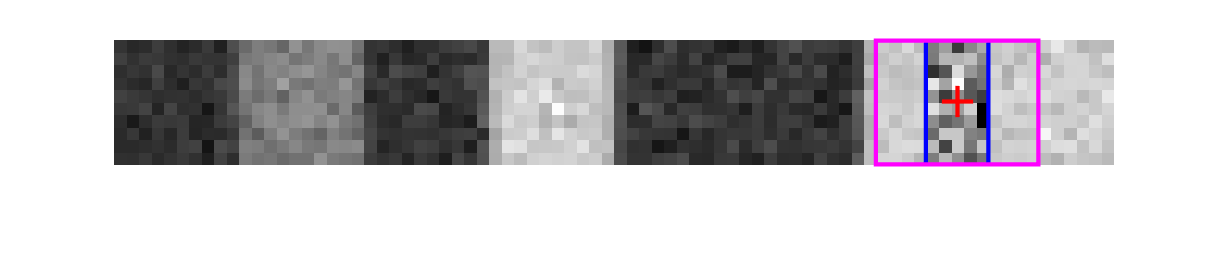
\includegraphics[width=0.49\textwidth]{figures/high_resolution_success_imL_fine.png}
        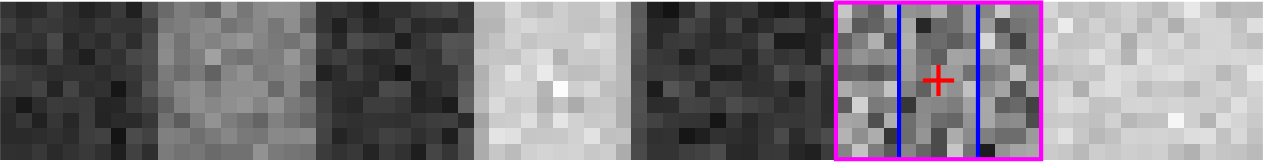
\includegraphics[width=0.49\textwidth]{figures/low_resolution_success_imL_fine.png}\\
        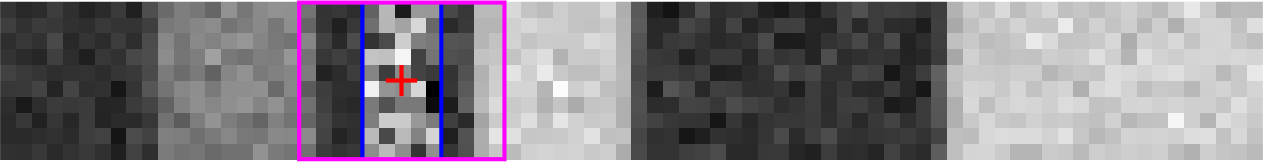
\includegraphics[width=0.49\textwidth]{figures/high_resolution_success_imR_fine.png}
        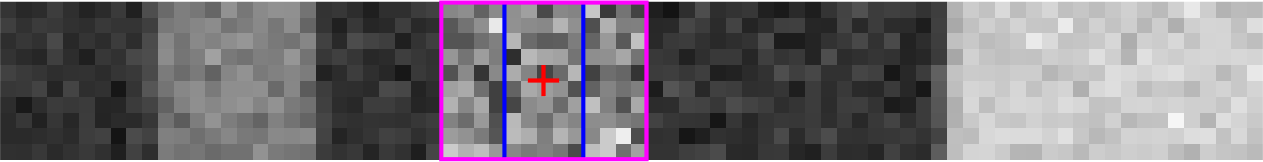
\includegraphics[width=0.49\textwidth]{figures/low_resolution_success_imR_fine.png}\\
        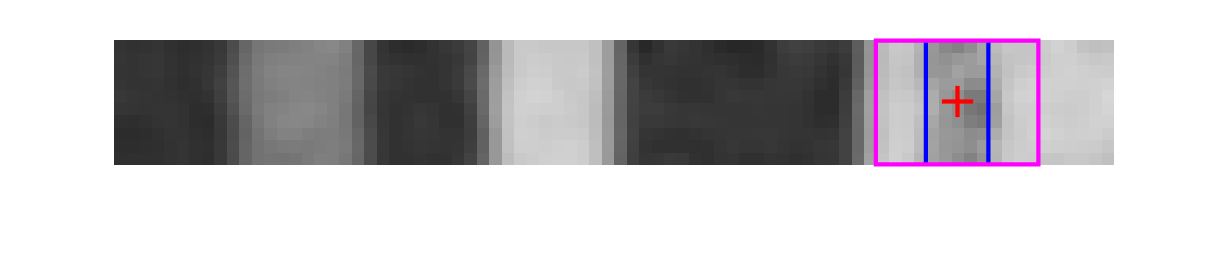
\includegraphics[width=0.49\textwidth]{figures/high_resolution_success_imL_coarse.png}
        
\includegraphics[width=0.49\textwidth]{figures/low_resolution_success_imL_coarse.png}\\
        
\includegraphics[width=0.49\textwidth]{figures/high_resolution_success_imR_coarse.png}
        
\includegraphics[width=0.49\textwidth]{figures/low_resolution_success_imR_coarse.png}\\
        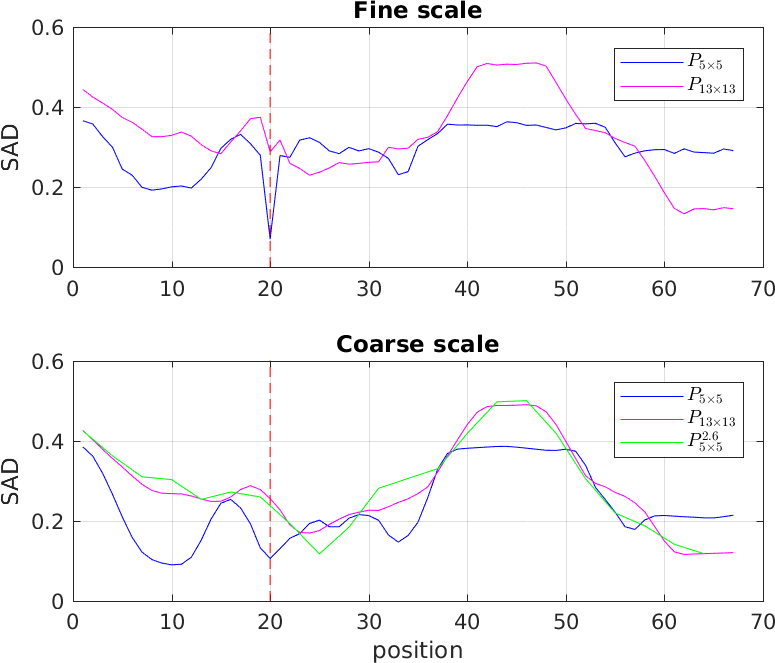
\includegraphics[width=0.49\textwidth]{paper/latex/figures/high_resolution_success_graph.png}
        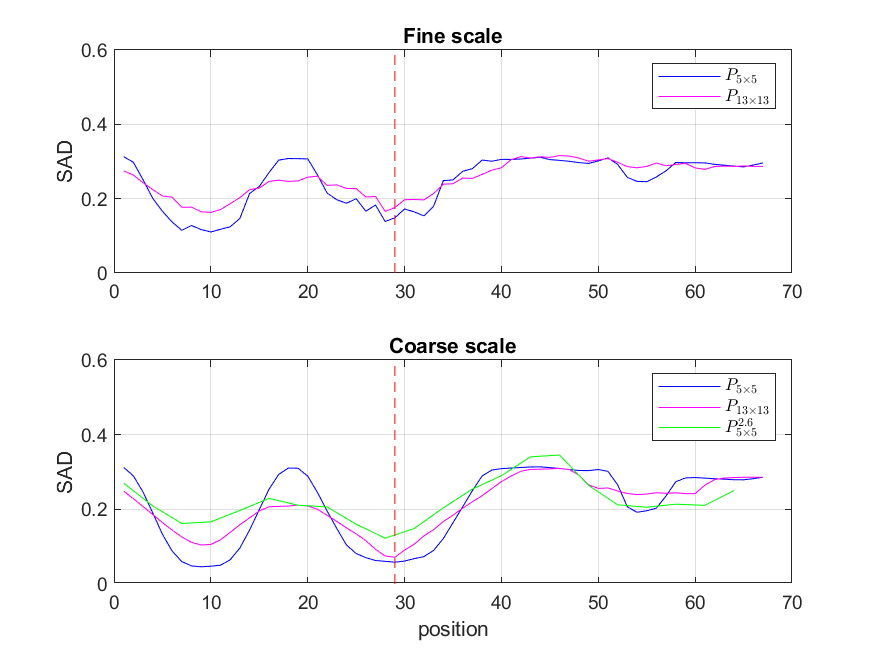
\includegraphics[width=0.49\textwidth]{paper/latex/figures/low_resolution_success_graph.png}\\
        
    \end{center}
    
    \caption{Simple artificial example. The left and the right column correspond to two different scenarios. In both columns, the first two images are the left and the right stereo view of the same 3D pattern, using orthographic projection. The next two images are the same views downscaled by a Gaussian filter. The red and blue bounding box corresponding to the two different patch sizes and the red cross to the reference point. In the graphs, we observe the curves of the matching process. The red dotted vertical line corresponds to the ground truth disparity.}
    \label{fig:multiscale_importance_2D}
\end{figure}

%%%%%%%%%%%%%%%%%%%%%%%%%%%%%%%%%%%%%%%%%%%%%%%%%%%%%%%%%%%%%%%%%%%%%%%%%%%%%%%%%%%%%%%%%%%%%%%%%%%%%%%%%%%%%%%%%%%%%%%%%%%%%%%%%%%%%%%%%%%%%%%%%%%

\section{Related Work}

Stereo reconstruction, as a core problem of computer vision, has been heavily studied over the last decades \cite{Barnard1982ComputationalStereo},\cite{Brown2003}. Scharstein and Szeliski \cite{Scharstein2001AAlgorithms} provided a generic taxonomy of the stereo vision methods based on their approach to the four fundamental tasks: (a) matching cost computation (b) cost aggregation (c) disparity computation/optimisation and (d) disparity refinement.

Up until recently, most methods relied on hand-engineered features for solving the matching cost and disparity computation problems. There have been proposed many different dissimilarity metrics, such as LoG, CENSUS \cite{Zabih1996ACorrespondence} and BRIEF \cite{Calonder2010}. The Graph Cut \cite{Kolmogorov}, \cite{Boykov2001} and belief propagation \cite{Klaus2006} methods managed to incorporate broader information in the final prediction. Hirschmuller minimised a global energy function with the Semi-Global-Matching (SGM) method \cite{Hirschmuller2008StereoInformation}. Geiger et. al \cite{Geiger2011EfficientMatching} attempted a Bayesian approach, using a prior distribution of the disparity image based on some robustly matched points.

Zagoruyko and Komodakis introduced the use of CNNs for comparing image patches \cite{zagoruyko2015learning}. Zbontar and LeCun \cite{Zbontar_2015_CVPR} used a similar CNN for computing the matching cost. They trained a binary CNN classifier to predict whether two patches correspond to the same 3D point. Their complete method, which involved some non-learnable parts (SGM), achieved state-of-the-art performance in the two well-known stereo datasets Middlebury \cite{Scharstein2014} and KITTI \cite{Menze2015ISA}. Luo et. al \cite{luo2016efficient} achieved comparable accuracy with a much faster implementation, by treating the matching cost as a multi-label classification problem. For the disparity refinement task, Shaked and Wolf \cite{shaked2017improved} proposed a disparity network which refined the initial disparity predictions, using confidence scores. Gidaris and Komodakis \cite{Gidaris2017DetectLabeling} proposed a CNN with three separate parts (Detect, Replace, Refine) for computing a refined disparity image. Seki and Pollefeys implemented a neural network version of the SGM algorithm, which learned from the data the penalty-scores of the discontinuities in the disparity map. 

All the approaches mentioned above used a CNN method for solving a particular subtask of the disparity estimation. On the contrary, Mayer et al. \cite{Mayer2016ALD} implemented an end-to-end CNN architecture (DispNet) for disparity estimation. The architecture included a contracting and an expanding part before making the final prediction. Apart from the proposed model, he also introduced a new synthetic dataset (SceneFlow) with approximately 35000 stereo images. Kendall et al. \cite{Kendall2017End-to-EndRegression} adjusted their architecture to the stereo vision geometry, by forming explicitly the Cost Matrix. They achieved that by introducing two novelities; (a) a 3D-convolutional network for processing the cost matrix and (b) a differentiable soft-argmin operator for the disparity estimation. 

Having achieved to formulate the stereo vision problem with an end-to-end CNN architecture, many works focused on exploiting semantic and context information. For this purpose, it was widely used the encoder-decoder architecture with residual connections, which contains many downscaling and upscaling layers.

Chang et al. \cite{Chang2018PyramidNetwork} designed a Spatial Pyramid Pooling (SPP) architecture for incorporating global information by aggregating context from different scales in the formation of the Cost Matrix. The Cost Matrix was then processed by a stacked-hourglass architecture (encoder-decoder structure). The Cascade Residual Network \cite{Pang2018CascadeMatching} has two subsequent stack-hourglass CNNs. The first one produces an initial disparity prediction that is used for warping the reference image and thus estimate an initial (unsupervised) error. Afterwards, the second CNN exploits this estimate for computing a refined prediction. EdgeStereo \cite{SongEdgeStereoResidual} focuses on the fine details that appear mainly around edges. Noticing that this area is error-prone due to occlusions, the network produces an edge-map which is subsequently used for measuring an edge-aware smoothness loss. DeepPruner \cite{du2019amnet} focuses on speeding-up the inference time by excluding some disparities and formulating a reduced Cost Matrix. This approach decreases the Search Space drastically and leads to an efficient prediction.




%%%%%%%%%%%%%%%%%%%%%%%%%%%%%%%%%%%%%%%%%%%%%%%%%%%%%%%%%%%%%%%%%%%%%%%%%%%%%%%%%%%%%%%%%%%%%%%%%%%%%%%%%%%%%%%%%%%%%%%%%%%%%%%%%%%%%%%%%%%%%%%%%%%
\section{The MSNet model}

In this section we analyse the building blocks (modules) that comprise the proposed MultiScaleNetwork (MSNet). Each module, named as $m_i$, is a procedure that gets a tensor as an input and produces another one as output. The learnable parts of each module are named as $f_i$ and the non-learnable ones as $g_i$. All modules are differentiable so that the backpropagation algorithm to be applicable end-to-end. Figure \ref{fig:cnn_architecture} provides an overview of the model.

\begin{figure}[!htbp]
    \centering
    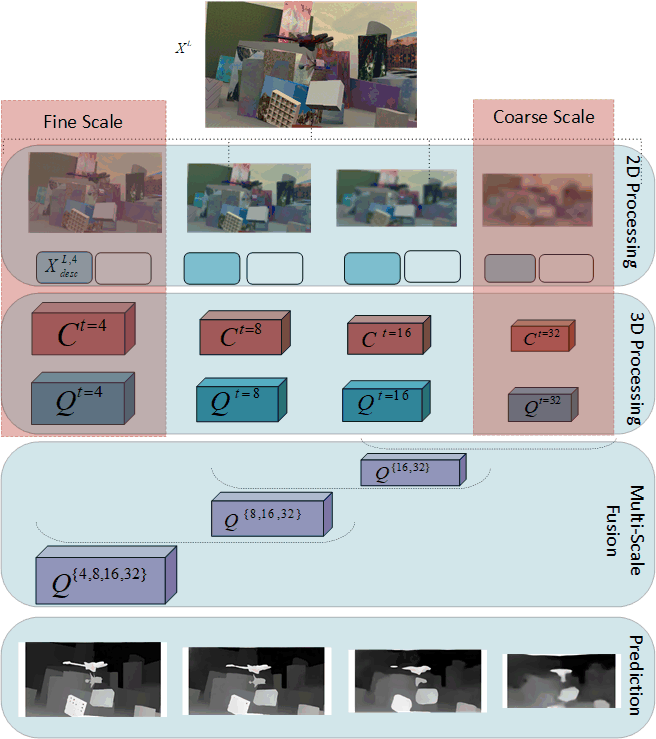
\includegraphics[width=0.7\textwidth, height=8cm]{figures/stereo_architecture.png}
    \caption{Overview of MSNet}
    \label{fig:cnn_architecture}
\end{figure}


\subsubsection{Downscaling Module - $m_1^t$}

The module $m_1^t: \mathbb{R}^{H \times W} \rightarrow \mathbb{R}^{\lceil \sfrac{H}{t} \rceil \times \lceil \sfrac{W}{t} \rceil }$ is applied separately to each stereo image for producing a downscaled stereo pair:

\begin{equation} \label{eq:g1}
    (X^{L,t}, X^{R,t}) = (m_1^t(X^L), m_1^t(X^R))
\end{equation}{}
%
The parameter $t$ is the downscaling and downsampling factor, as defined in equations \ref{eq:t_param1}, \ref{eq:t_param2}. The module $m_1^t$ is a two-step procedure; firstly each stereo image $X^{\{L|R\}}$ is convolved with the discrete Gaussian kernel of equation \ref{eq:g1_kernel} in order to remove the high-frequency components, and afterwards the downscaling is performed with bilinear downsampling interpolation.

\begin{gather} \label{eq:g1_kernel}
    k(x, y, \sigma) = \frac{1}{2\pi\sigma^2} \cdot e^{\sfrac{-(x^2 + y^2)}{2\sigma^2}}, \quad \sigma = \sfrac{t}{3}
    % x,y \in \{-\lceil 4*\sigma + 0.5 \rceil, ..., \lceil 4*\sigma + 0.5 \rceil\}, \sigma = \sfrac{t}{3}
\end{gather}

\subsubsection{Feature Extraction - $m_2$}

The module $m_2: \mathbb{R}^{H \times W \times 3} \rightarrow \mathbb{R}^{H \times W \times K}$ extracts local features from the raw stereo images, through a CNN ($f_2$). The feature extraction process is repeated separately at each scale:

\begin{equation} \label{eq:f_1}
    m_2:(X^{L,t}_{desc}, X^{R,t}_{desc}) = (f_2(X^{L,t}), f_2(X^{R, t}))
\end{equation} 

\subsubsection{Comparison Volume - $m_3$} The module $m_3$
$$m_3:(\mathbb{R}^{H \times W \times K}, \mathbb{R}^{H \times W \times K}, \mathbb{R}^{H \times W \times 3}) \rightarrow \mathbb{R}^{D \times H \times W \times (K+3)}$$ forms the Comparison Volume ($C^t$), by zipping the comparison information into a 3D tensor. Normally, the Comparison Volume is formed by simply concatenating the descriptors in each disparity position. This approach introduces significant redundancy; from the $D \times H \times W \times 2K$ values of the Comparison Volume only the $H \times W \times 2K$ are unique. For reducing such redundancy, we design a new comparison metric between two scalar features:

\begin{equation} \label{eq:m}
    l: \mathbb{R}^2 \rightarrow \mathbb{R}: l(a_1, a_2) = \frac{|a_1| + |a_2|}{2} \cdot e^{-|a_1 - a_2|}    
\end{equation}

 The first term $\frac{|a_1| + |a_2|}{2}$ measures the existence of a feature in each patch separately ($0$ signifies non-existence) and the second term $e^{-|a_1 - a_2|} \in (0,1]$ measures the coexistence of the feature in both patches. Finally, we concatenate the raw left image $X^L$, in order to propagate the raw image in the subsequent layers. The formulation of the comparison volume is described in equation \ref{eq:comparison_volume}:

\begin{equation}\label{eq:comparison_volume}
C^t[d, x, y, i] = 
    \begin{cases}
        l( X^{L, t}_{desc}[x,y,i], X^{R, t}_{desc}[x-d,y, i]) &\quad ,i \leq K \\
        X^{L,t}[x,y,i-K] &\quad ,i > K
     \end{cases}
\end{equation}{}  


\subsubsection{Comparison Volume Processing - $m_4$} The module $m_4: \mathbb{R}^{D \times H \times W \times K} \rightarrow \mathbb{R}^{D \times H \times W \times K}$ is a CNN ($f_4$) with 3D convolutional layers, that incorporates local information along all 3 dimensions (the 2 spatial ones $x,y$ and the disparity $d$) for refining the Comparison Volume. It ouptuts a same-dimension volume $Q^t$:

\begin{equation}
    m_4: Q^t = f_4(C^t)
\end{equation}


\subsubsection{Multiscale Fusion - $m_5$}

The module $m_5$ is responsible for exploiting the information from different scales and combine it in a single tensor. The procedure takes place recursively in pairs of two Comparison Volumes, from coarse to fine scales. A trilinear upsampling layer $g_3^t: \mathbb{R}^{D \times H \times W \times K} \rightarrow \mathbb{R}^{tD \times tH \times tW \times K}$ is applied to the low-dimension Comparison Volume before a CNN ($f_5$) with 3D-Convolutional layers merge the information of the two scales into one tensor, as describe in equation \ref{eq:two_scale_fusion}. Repeating this procedure recursively as shown in algorithm \ref{alg:multi_scale_fusion} leads to a single Comparison Volume, that incorporates information from all separate scales. The implementation of the scale fusion procedure as a recursive merging is the key idea that enables our network to be readjustable:

\begin{equation} \label{eq:two_scale_fusion}
Q^{ \{ t_i, \cdot \cdot \cdot, t_{n} \} } = f_5(Q^{t_i} \oplus g_5^{\sfrac{t_i}{t_{i-1}} }(Q^{ \{ t_{i-1}, \cdot \cdot \cdot, t_n \} }))
\end{equation}

\begin{algorithm}
\caption{Multi-scale fusion - Module $m_5$}\label{alg:multi_scale_fusion}
\begin{algorithmic}[1]
\Procedure{multi scale fusion}{$ Q^{t_0}, Q^{t_1}, \cdot \cdot \cdot, Q^{t_n} $} $\rightarrow Q^{\{t_0, t_1, \cdot \cdot \cdot, t_n\}}$ 
\State $Q \gets Q^{t_n}$ \Comment{Initialize}
\For { \texttt{i=n-1;-1;0} }
\State $Q \gets g_3^{\sfrac{ t_{i+1} }{ t_i } }(Q)$ \Comment{3D Upsampling}
\State $Q \gets Q^{t_i} \oplus Q$ \Comment{Concatenation}
\State $Q \gets f_5(Q)$ \Comment{Merge information}
\EndFor
\State \Return $Q^{\{t_0, t_1, \cdot \cdot \cdot, t_n\}} \gets Q$ \Comment{Result}
\EndProcedure
\end{algorithmic}
\end{algorithm}


\subsubsection{Module For Depth Prediction - $m_6$}

The module $m_6^t: \mathbb{R}^{\sfrac{D}{t} \times \sfrac{H}{t} \times \sfrac{W}{t} \times K} \rightarrow \mathbb{R}^{D \times H \times W}$ implements the final disparity prediction. It consists of three sequential parts: (a) a CNN with 3D-convolutional layers $f_6: \mathbb{R}^{D \times H \times W \times K} \rightarrow \mathbb{R}^{D \times H \times W}$ that assigns a probability in each possible disparity $S^{\{ t_0, \cdot \cdot \cdot, t_n \}} = f_6(Q^{\{t_0, t_1, \cdot \cdot \cdot, t_n\}})$, (b) a trilinear upsampling layer for upsampling $S$ in the initial dimensions $D \times H \times W$ and finally (c) a softmax operator applied along the disparity dimension, for obtaining the final prediction $\hat{Y}^{\{t_0, t_1, \cdot \cdot \cdot, t_n\}}$.

\subsubsection{Putting all pieces together}

Before the execution of a single prediction, a set of processing scales $T = \{t_0, ..., t_n\}$ must be defined. The modules $m_1, m_2, m_3, m_4$ operate separately on the stereo pair for producing a single scale Comparison Volume $Q^t$. Subsequently, the module $m_5$ combines the information from all single-scale volumes to a single tensor $Q^{t_0, ..., t_n}$ and the module $m_6$ makes the disparity prediction. The whole prediction procedure is summarized in algorithm \ref{alg:MSNET}.

% It is important to notice that the learnable parts of our network are scale-independent; they are trained to operate independently of the specific scale of the input. This property gives the freedom to define the set of processing scales $T$ at test time, according to the needs and the computational resources of each application. A more extended experimentation of how the accuracy and the efficiency of the network varies as processing scales are added or remove is presented in the next section. 

\begin{algorithm}
\caption{MultiScaleNetwork (MSNet)}\label{alg:MSNET}
\begin{algorithmic}[1]
\State $T \gets \{ t_0, t_1, ... , t_n\}$ \Comment{Define Processing Scales}
\Procedure{MSNet}{$ X^L, X^R, T$} $\rightarrow \hat{Y}$ 
\For { \texttt{t in T} }
\State $(x^{L,t},  x^{R,t}) \gets (m_1^t(X^L),m_1^t(X^R)) $ \Comment{Downscaling}
\State $(x^{L,t}_{desc}, x^{R,t}_{desc}) \gets (m_2(X^L), m_2(X^L))$ \Comment{Features}
\State $C^{t} \gets m_3(X^{L,t}_{desc}, X^{R,t}_{desc}, X^{L,t})$ \Comment{Comparison Volume}
\State $Q^{t} \gets m_4(C^{t})$ 
\EndFor
\State $Q^{\{t_0, t_1, \cdot \cdot \cdot, t_n\}} \gets m_5(Q^{t_0}, Q^{t_1}, \cdot \cdot \cdot, Q^{t_n})$ \Comment{MultiScaleFusion}
\State $\hat{Y}^{\{ t_0, \cdot \cdot \cdot, t_n \}} = m_6(Q^{\{t_0, t_1, \cdot \cdot \cdot, t_n\}}) $ \Comment{Prediction}
\State \Return $\hat{Y}^{\{ t_0, \cdot \cdot \cdot, t_n \}} $
\EndProcedure
\end{algorithmic}
\end{algorithm}

\subsection*{Cnn architectures}

The learnable parts of MSNet ($f_2, f_4, f_5, f_6$) are four CNNs, that follow similar architecture. A residual connection, which comprises of two blocks of Batch Normalization, ReLU and Convolution in sequential order with a residual connection added to the output, is used as a fundamental building block in all architectures. In $f_2$, which operates on 2D inputs, the convolution is 2D (i.e. kernel size 3x3), whereas for $f_4, f_5, f_6$ the convolution is 3D, applied along the disparity dimension as well (kernel size 3x3x3).


\begin{table}
    \centering
    \resizebox{0.7\textwidth}{!}{
    \begin{tabular}{ c|c|c|c|c }
    \textbf{Module} & \textbf{Structure} & \textbf{Input} & \textbf{Output} & \textbf{Parameters} \\
    
    \hline
    
    \multirow{2}{*}{$f_2$} & BN+ReLU+Conv2D & HxWx3 & HxWx32 & \multirow{2}{*}{74592} \\
    & 4xRes2D & HxWx32 & HxWx32 &
    \\

    \hline

    \multirow{2}{*}{$f_4$} & BN+ReLU+Conv3D & DxHxWx64 & DxHxWx32 & \multirow{2}{*}{196128} \\
    & 3xRes3D & DxHxWx32 & DxHxWx32 & \\
    
    \hline
    
    \multirow{3}{*}{$f_5$} & BN+ReLU+Conv3D & DxHxWx64 & DxHxWx64 & 
    \multirow{3}{*}{331776}  \\
    & BN+ReLU+Conv3D & DxHxWx64 & DxHxWx32 & \\
    & 3xRes3D & DxHxWx32 & DxHxWx32 & \\

    \hline
    
    \multirow{3}{*}{$f_6$} & BN+ReLU+Conv3D & DxHxWx64 & DxHxWx64 &
    \multirow{3}{*}{139104} \\
    & 2xRes3D & DxHxWx32 & DxHxWx32 & \\
    & BN+ReLU+Conv3D & DxHxWx32 & DxHxW & \\

    \hline
    MSNet & & HxWx3 & HxW & 741600
    \end{tabular}
    }
    \caption{Description of CNN architectures}
    \label{tab:learnable_models}
\end{table}

%%%%%%%%%%%%%%%%%%%%%%%%%%%%%%%%%%%%%%%%%%%%%%%%%%%%%%%%%%%%%%%%%%%%%%%%%%%%%%%%%%%%%%%%%%%%%%%%%%%%%%%%%%%%%%%%%%%%%%%%%%%%%%%%%%%%%%%%%%%%%%%%%%%
\section{Experimental Evaluation}

The experimental evaluation is organized in four parts; In the first part (4.1), MSNet is compared with the State-of-the-art methods, in terms of accuracy and efficiency. In the second part (4.2, 4.3), we set up an internal benchmark for questioning the major architectural choices of MSNet; we evaluate some alternative models that share similar designing principles with the MSNet (i.e. same backbone architecture) with crucial modifications in the decisive details we want to measure. In the third part (4.4), we observe how MSNet behaves under different sets of processing scales, quantifying the trade-off between accuracy and efficiency. In the final part (section 4.5), we illustrate how MSNet has learned to incorporate information from all processing scales in an incremental fashion.

All experiments are based on the synthetic SceneFlow dataset \cite{MIFDB16}, which consists of dense ground truth disparity images (H=540, W=960). The 
default training/test set split (35454 training vs 4370 testing images) has been followed in all benchmarks. For the evaluation of the models, we use (a) the End-Point-Error (EPE) metric - mean absolute prediction error - and (b) the percentage ($\text{PCG}_k$) metric - the percentage of points with absolute error over $k$ pixels. All models have been trained from scratch in a GeForce GTX 1080, with random initialization following the fan-in approach ($\theta \sim N(0,\sigma=\sqrt{\sfrac{2}{n}})$) \cite{He2015}. The training images are randomly cropped in (H=256, W=512) patches and normalized with ImageNet preprocessing statistics (mean, std). The Adam optimizer ($\beta_1 = 0.9, \beta_2=0.999$) with a learning rate of 0.001 was used for 15 epochs, with batch size set at 2. At the training phase of MSNet, the processing scales were preset to $T= \{2^2, 2^3, 2^4, 2^5\}$ and the final loss $L$ was a weighted sum of the EPE loss computed after incorporating each processing scale:

\begin{gather}
\textit{Loss} := \dfrac{1}{2}L^{\{t_0, t_1, t_2, t_3\}} +  \dfrac{1}{6}L^{\{t_1, t_2, t_3\}} + \dfrac{1}{6}L^{\{t_2, t_3\}} + \dfrac{1}{6}L^{\{t_3\}}\\
\text{where:} \; \ L^{\{t_i, ..., t_j\}} = |\hat{Y}^{\{t_i, ..., t_j\}} - Y |    
\end{gather}{}


\subsection{Comparison with the State-Of-The-Art}

The comparisons are based on three criteria; (a) accuracy (EPE, $\text{PCG}_3$) (b) efficiency (runtime) and (c) the number of free parameters. The efficiency is measured as the runtime for a single prediction. The number of free parameters is manifested since it is related to the memory resources and the amount of training data demanded by each model. In table \ref{tab:results}, we observe that MSNet achieves competitive performance (i.e. $1.017$px EPE compared to the $0.74$px in in the SOTA \cite{du2019amnet}) even though it uses much less free parameters and it is more efficient than (almost) all its competitive networks. Specifically, only \cite{Duggal2019ICCV} outperforms MSNet both in terms of accuracy and efficiency; models \cite{cheng2018learning}, \cite{du2019amnet}, \cite{zhang2019ga} are more accurate but less efficient and they use more free parameters. The only model (apart from \cite{Duggal2019ICCV}) that is more efficient than MSNet is \cite{Mayer2016ALD}, but is less accurate.

\begin{table}
    \centering
    \resizebox{0.6\textwidth}{!}{%
    \begin{tabular}{ c|c|c|c|c }
    Method & Parameters(M) & Runtime(s)& EPE(px)& $\text{PCG}_3$(\%) \\
    
    \hline
    \multicolumn{5}{c}{ \textbf{Our benchmark - IMS architectures} } \\
    \hline
    MSNet & \textbf{0.741} & 0.32 & 1.017 & 3.98 \\
    \hline
    OneRes (S) & 0.463 & 0.11 & 1.508 & 6.11 \\
    MRes2d (S) & 0.659 & 0.10 & 1.671 & 6.98 \\
    MRes3d (S) & 0.514 & 0.15 & 1.504 & 5.86 \\
    MRes2d3d (S) & 0.677 & 0.3 & 1.897 & 8.078 \\
    \hline
    OneRes (B) & 1.608 & 0.22 & 1.37 & 5.53 \\
    MRes2d (B) & 1.458 & 0.17 & 1.32 & 5.43 \\
    MRes3d (B) & 1.682 & 0.21 & 1.322 & 5.11 \\
    MRes2d3d (B) & 1.772 & 0.32 & 1.613 & 6.67 \\
    \hline
    \multicolumn{5}{c}{ \textbf{Our benchmark - Free weights} } \\
    \hline
    Free2d & 0.969 & 0.24 & 1.126 & 4.33 \\
    Free3d & 2.75 & 0.33 & \textbf{0.882} & \textbf{3.48} \\
    Free2d3d & 2.974 & 0.33 & 1.107 & 4.36 \\
    \hline
    \multicolumn{5}{c}{ \textbf{SOTA} } \\
    \hline
    PSMNet\cite{Chang2018PyramidNetwork} & 5.2 & 0.45 & 1.09 & - \\
    CRL\cite{Pang2018CascadeMatching} & - & 0.47 & 1.32 & - \\
    DispNetC\cite{Mayer2016ALD} & - & \textbf{0.06} & 1.68 & - \\
    GC-Net\cite{Kendall2017End-to-EndRegression} & 3.5 & 0.95 & 2.51 & 9.34 \\
    Edge-Stereo\cite{SongEdgeStereoResidual} & - & - & 1.12 & 4.99 \\
    CSPN\cite{cheng2018learning} & 250 & 0.5 & 0.78 & - \\
    GA-Net\cite{zhang2019ga} & 2.3 & 1.5 & 0.84 & - \\
    AMNet\cite{du2019amnet} & 4.37 & - & \textbf{0.74} & - \\
    \textbf{DeepPruner}\cite{Duggal2019ICCV} & - & 0.6 & 0.97 & -\\
    \hline
    \end{tabular}%
    }
    \caption{Model comparison on the SceneFlow dataset. The EPE and PCG of MSNEt are measured for the default set of scales $T=\{2^2, 2^3, 2^4, 2^5\}$.}
    \label{tab:results}
\end{table}

\begin{figure}
    \begin{center}
        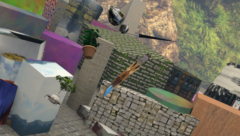
\includegraphics[width=0.24\textwidth,height=0.08\textwidth,clip]{figures/imL_0.png}
        
\includegraphics[width=0.24\textwidth,height=0.08\textwidth,clip]{figures/imL_1.png}
        
\includegraphics[width=0.24\textwidth,height=0.08\textwidth,clip]{figures/imL_2.png}
        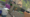
\includegraphics[width=0.24\textwidth,height=0.08\textwidth,clip]{figures/imL_3.png}
        \\
        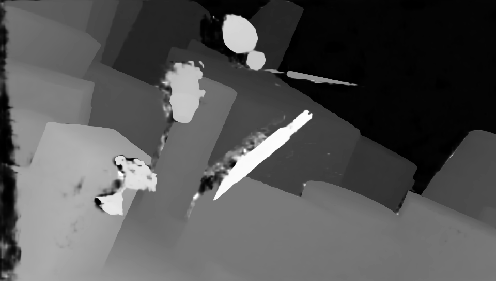
\includegraphics[width=0.24\textwidth,height=0.08\textwidth,clip]{figures/pred_0.png}
        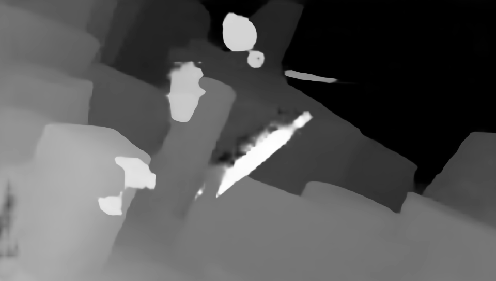
\includegraphics[width=0.24\textwidth,height=0.08\textwidth,clip]{figures/pred_1.png}
        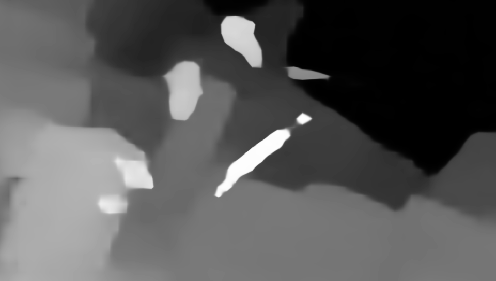
\includegraphics[width=0.24\textwidth,height=0.08\textwidth,clip]{figures/pred_2.png}
        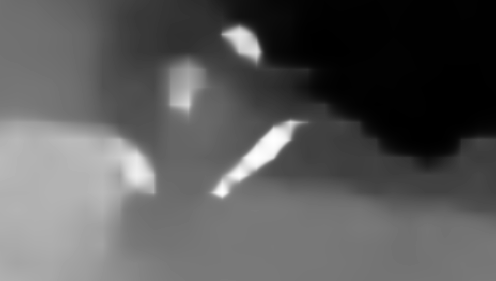
\includegraphics[width=0.24\textwidth,height=0.08\textwidth,clip]{figures/pred_3.png}
        \\
        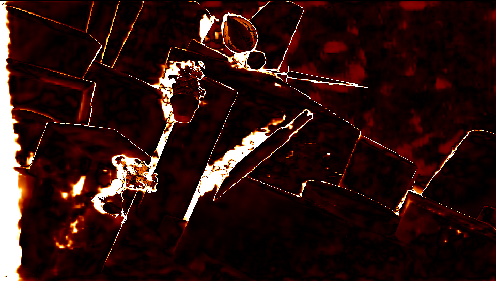
\includegraphics[width=0.24\textwidth,height=0.08\textwidth,clip]{figures/pred_0_err.png}
        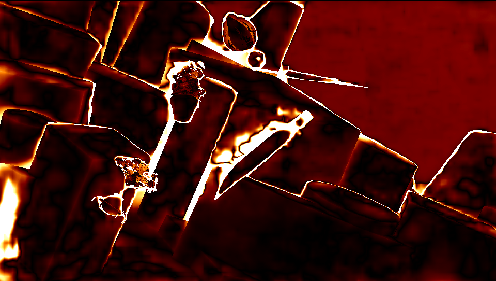
\includegraphics[width=0.24\textwidth,height=0.08\textwidth,clip]{figures/pred_1_err.png}
        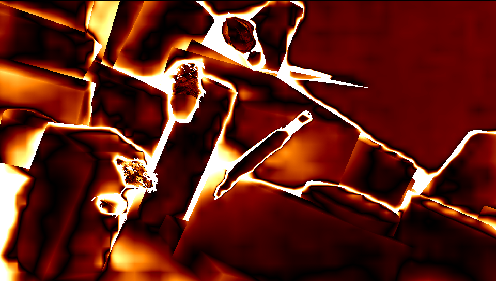
\includegraphics[width=0.24\textwidth,height=0.08\textwidth,clip]{figures/pred_2_err.png}
        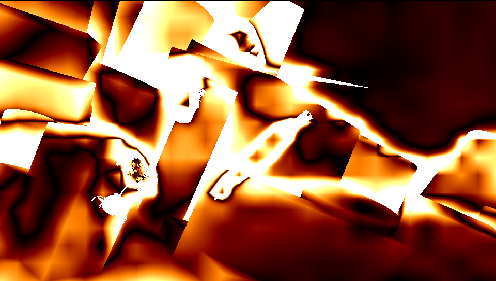
\includegraphics[width=0.24\textwidth,height=0.08\textwidth,clip]{figures/pred_3_err.png}
        \\
        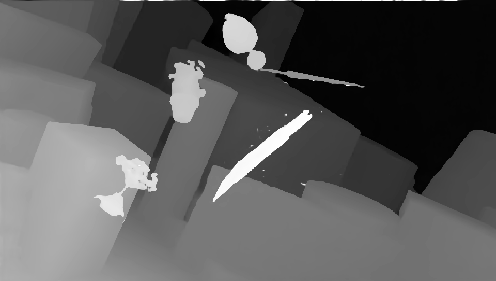
\includegraphics[width=0.24\textwidth,height=0.08\textwidth,clip]{figures/pred_comb_0.png}
        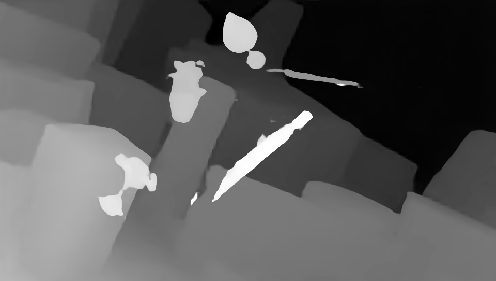
\includegraphics[width=0.24\textwidth,height=0.08\textwidth,clip]{figures/pred_comb_1.png}
        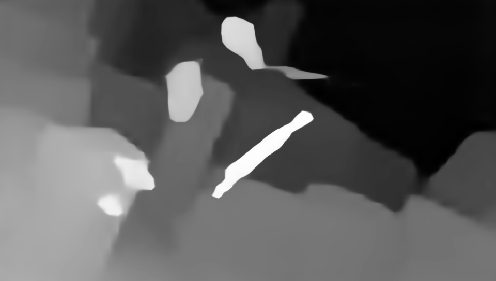
\includegraphics[width=0.24\textwidth,height=0.08\textwidth,clip]{figures/pred_comb_2.png}
        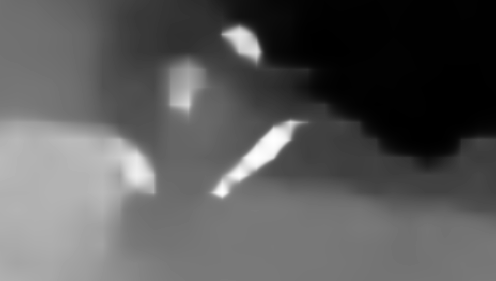
\includegraphics[width=0.24\textwidth,height=0.08\textwidth,clip]{figures/pred_comb_3.png}
        \\
        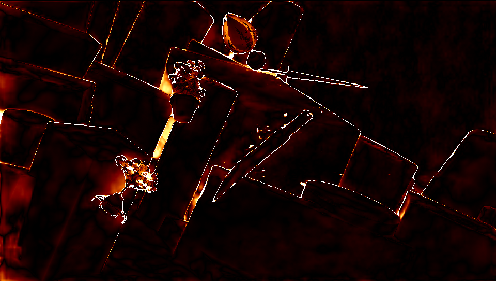
\includegraphics[width=0.24\textwidth,height=0.08\textwidth,clip]{figures/pred_comb_0_err.png}
        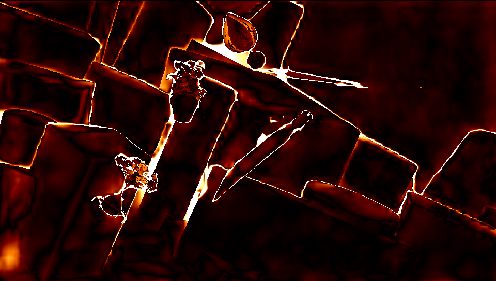
\includegraphics[width=0.24\textwidth,height=0.08\textwidth,clip]{figures/pred_comb_1_err.png}
        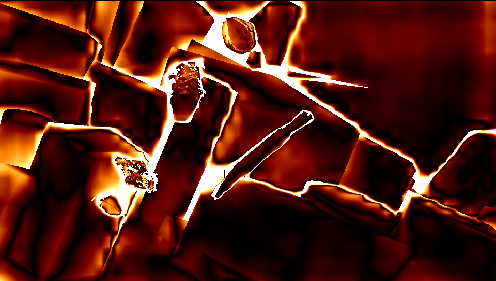
\includegraphics[width=0.24\textwidth,height=0.08\textwidth,clip]{figures/pred_comb_2_err.png}
        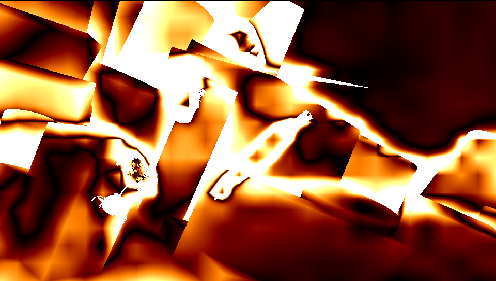
\includegraphics[width=0.24\textwidth,height=0.08\textwidth,clip]{figures/pred_comb_3_err.png}
    \end{center}
    \caption{Illustration of the prediction process along processing scales. The first row (left to right) contains the left image along all scales $X^{L,t} : t \in \{2^2, 2^3, 2^4, 2^5\}$. The second and the third row contain the \textbf{single scale} predictions $\hat{Y}^{t}$ and absolute error images $E^{t}$. The last two rows contain the \textbf{multiscale} predictions (processing scales are added incrementally as we move from right to left) and the corresponding error images. We can observe the limitations of single-scale predictions; coarse scales fail in describing the details between objects while fine scales suffer from instabilities. On the other hand, the multiscale prediction combines the benefits of both worlds; it starts with a rough estimation of the disparity image, incorporating higher-resolution details as it integrates fine scales.}
    \label{fig:EMAPs}
\end{figure}

\subsection{The Effect Of Reinforcing Multi-Scale Processing}

In this section, we question whether enforcing the multi-scale processing explicitly, as we do in MSNet, is advantageous over using multi-scale processing internally as part of the CNN architecture. For this reason, we design four new models that follow the MSNet designing principles, but without reinforcing multi-scale processing explicitly; instead, they follow the hourglass architecture (i.e. encoder-decoder) which is the proposed method, by the literature, for applying multi-resolution processing internally. We design the following four architectures; OneRes operates only on the initial resolution, MRes2d uses the hourglass model only in the 2D-processing part ($f_2$), MRes3d only in the 3D-processing part ($f_4, f_5, f_6$) and finally MRes2d3d in both the 2D and 3D processing part ($f_2, f_4, f_5, f_6$). For each of the 4 CNNs, we create two versions; the small (S) version with the same order of free parameters as the MSNet (approximately $600K$) and the big (B) version which has as many parameters as the GPU's memory allows (approximately $1.6M$). For clarity, we call all these new models with the common name Implicit Multi-Scale (IMS) architectures.

In figure \ref{fig:mae_SFNvsGenericNets} (Left), we observe that MSNet outperforms both versions of the IMS architectures, which is a strong indicator that reinforcing multi-scale processing explicitly is beneficial for the problem of depth estimation. As expected, all big (B) networks outperform small (S) ones.

\begin{figure}[!htbp]
    \centering
    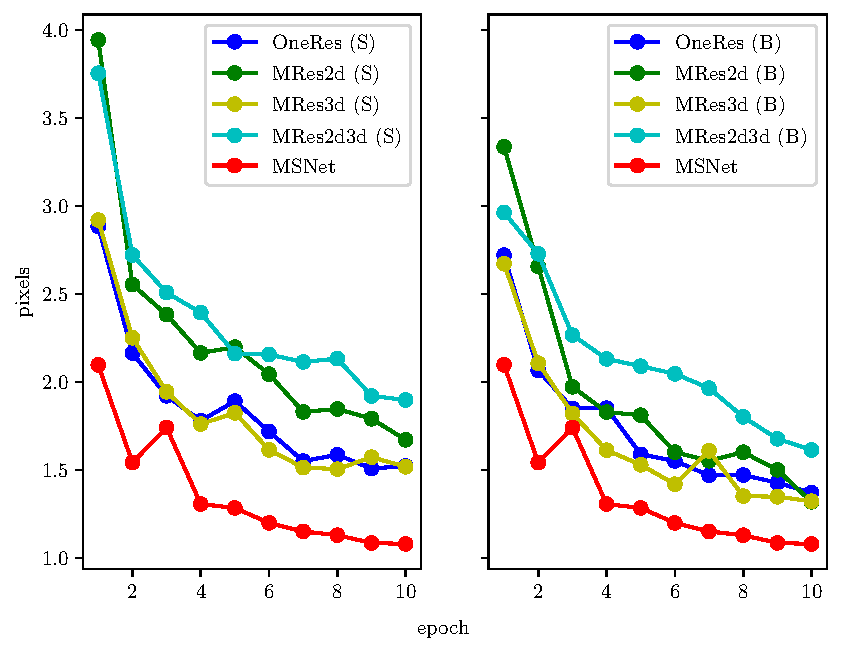
\includegraphics[width=0.49\textwidth, height=0.3\textwidth]{figures/freiburg_msnet_vs_monolithic_mae.pdf}
    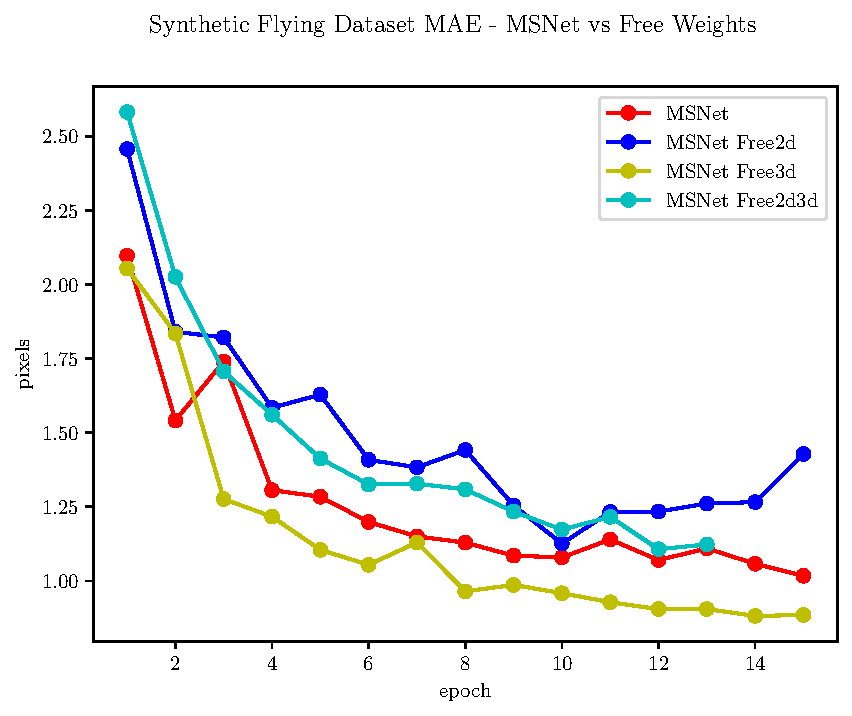
\includegraphics[width=0.49\textwidth, height=0.3\textwidth]{figures/freiburg_msnet_vs_free_weights_mae.pdf}
    \caption{(Left) Comparison of MSNet with IMS architectures. (Right) Comparison of MSNet with Free Weight Networks.}
    \label{fig:mae_SFNvsGenericNets}
\end{figure}

\subsection{The Cost of Sharing Weights}

MSNet obtains its fundamental advantage of being adjustable by repeating its learnable-parts in between the different processing scales. An important question that arises is how much is the cost in terms of accuracy for gaining such scalability; what is the corresponding EPE if we use the MSNET architecture without weight sharing (i.e. train different learnable parts at each scale, instead of repeating the same building blocks). For answering this question, we create a second internal benchmark, by implementing three new CNN architectures; The \textit{MSNet-Free2d} has free weights only in the 2D-processing part (doesn't repeat $f_2$ blocks), \textit{MSNet-Free3D} has free weights only in the 3D-processing part (doesn't repeat $f_4, f_5, f_6$ building blocks) and, finally, \textit{MSNet-Free2D3D} has free weights in both parts. Since these new architectures are no longer adjustable, we predefine the processing scales to be $T = \{2^2, 2^3, 2^4, 2^5\}$. The evaluation on the SceneFlow dataset is presented in figure \ref{fig:mae_SFNvsGenericNets}. We observe that training different CNNs for each scale of the 3D-processing part ($f_5, f_5, f_6$) leads to superior performance. This experimental observation indicates that the MultiScaleFusion algorithm, which incorporates the different scales in pairs of two, achieves a suboptimal solution. This can be explained due to two reasons; (a) the number of free weights in \textit{MSNet Free-*} models is increased by a factor of $4x$ compared to MSNet and (b) MultiScaleFusion's designing principle of incorporating only one new scale at a time, deprives the beneficial global view of all scales simultaneously. Even though \textit{MSNet-Free3D} outperforms our proposed model, such approach cancels the fundamental scalability advantage of MSNet.

\subsection{MSNet evaluation on different scale combinations}

The fundamental advantage of MSNet compared to other architectures is the ability to get tuned between accuracy and efficiency at test time. In figure \ref{fig:msnet_scales_evaluation}, we measure how three fundamental properties of MSNet (a) accuracy (b) stability and (c) efficiency vary under different scale combinations. For the accuracy, measured through the EPE, we can observe two interesting properties; (a) combined scales have different impact on the accuracy than when used individually (i.e. T = $\{t_0=4,t_1=32\}$ has the best performance among all two-scale combinations, though $t_0=4$, $t_1=32$ have the worst accuracy individually) and (b) adding an additional scale in a set always improves accuracy. Stability is quantified through the standard deviation $\sigma$ of the EPE. We observe that coarse scales are in general more stable and that stability increases as we add more processing scales. Finally, we observe that the runtime increases exponentially as we add high-resolution scales (e.g the set $T = \{t_0=4\}$ is less efficient than $T = \{t_0=8, t_1 = 16, t_2 =32\}$)

In general terms, MSNet has a robust behavior under different scale combinations. Adding a new processing scale increases the accuracy. Excluding the computational demanding fine scales, improves the efficiency exponentially, without an accuracy crumble. As a characteristic example, the combination $T = \{8, 32\}$ has EPE $<2$ px and execution time $<0.05s$. 

\begin{figure}[htb!]
    \centering
    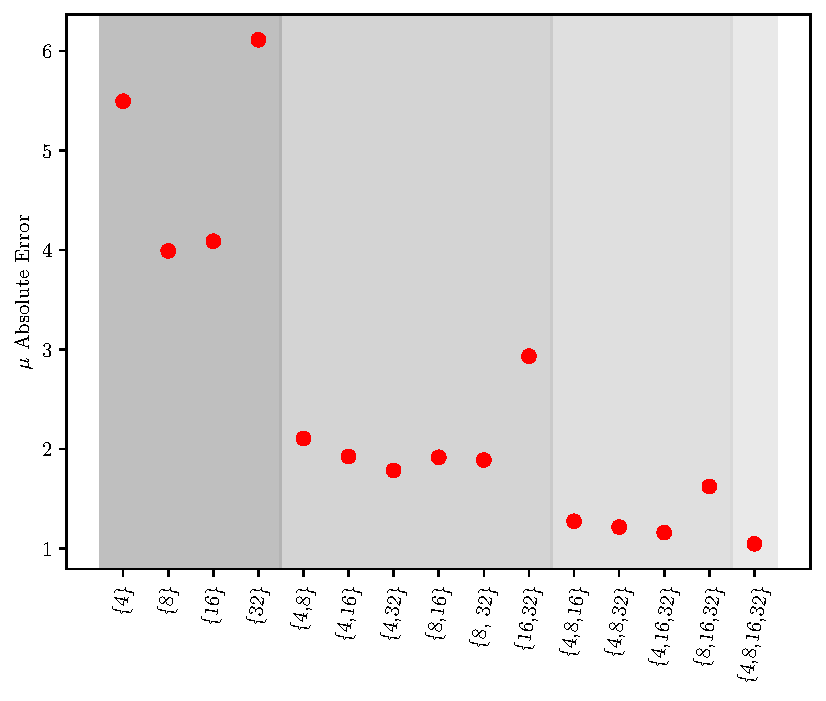
\includegraphics[width=0.3\textwidth]{figures/msnet_scales_evaluation1.pdf}
    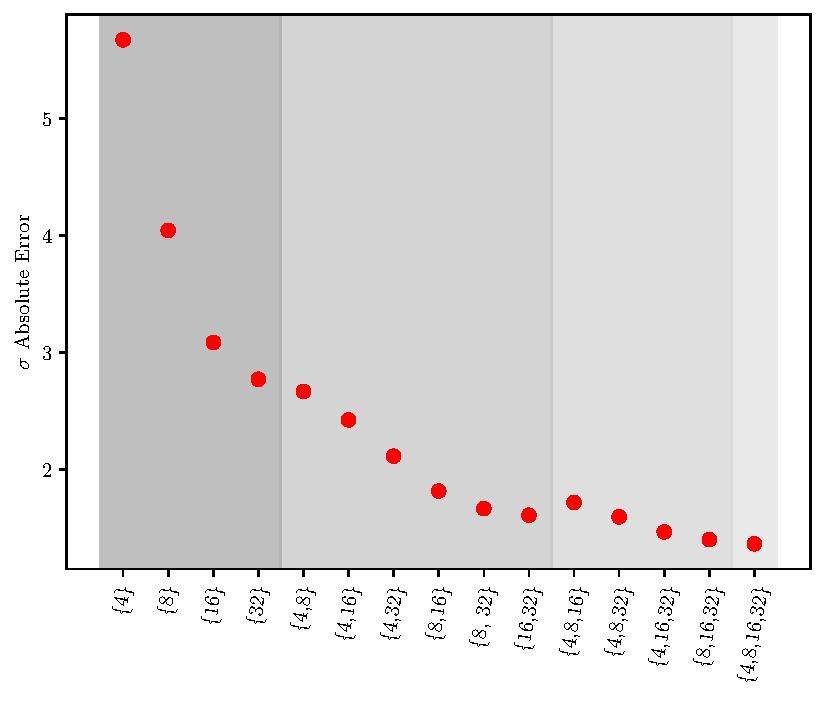
\includegraphics[width=0.3\textwidth]{figures/msnet_scales_evaluation2.pdf}
    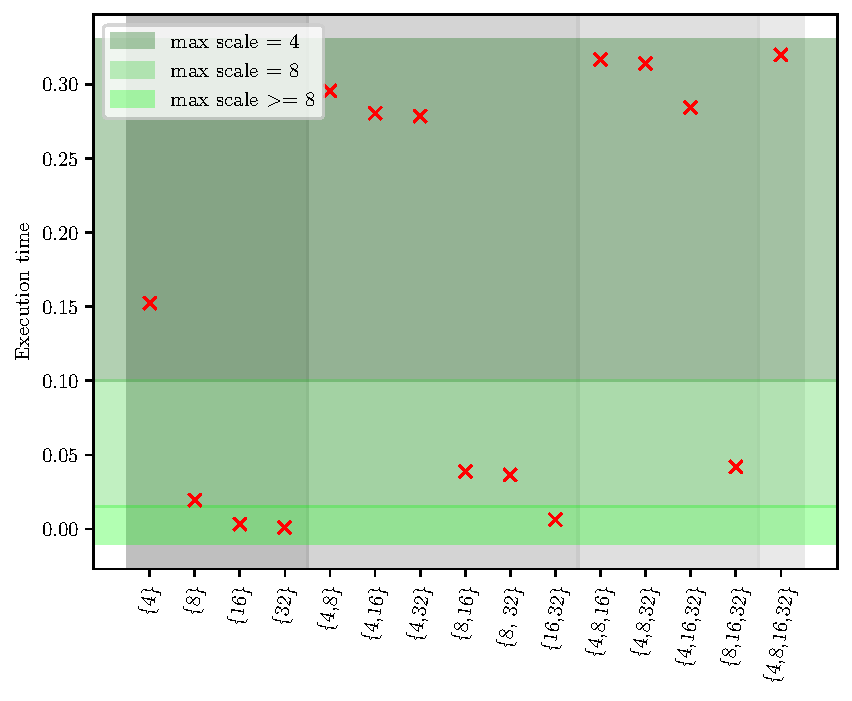
\includegraphics[width=0.3\textwidth]{paper/latex/figures/msnet_inference_times.pdf}
    % 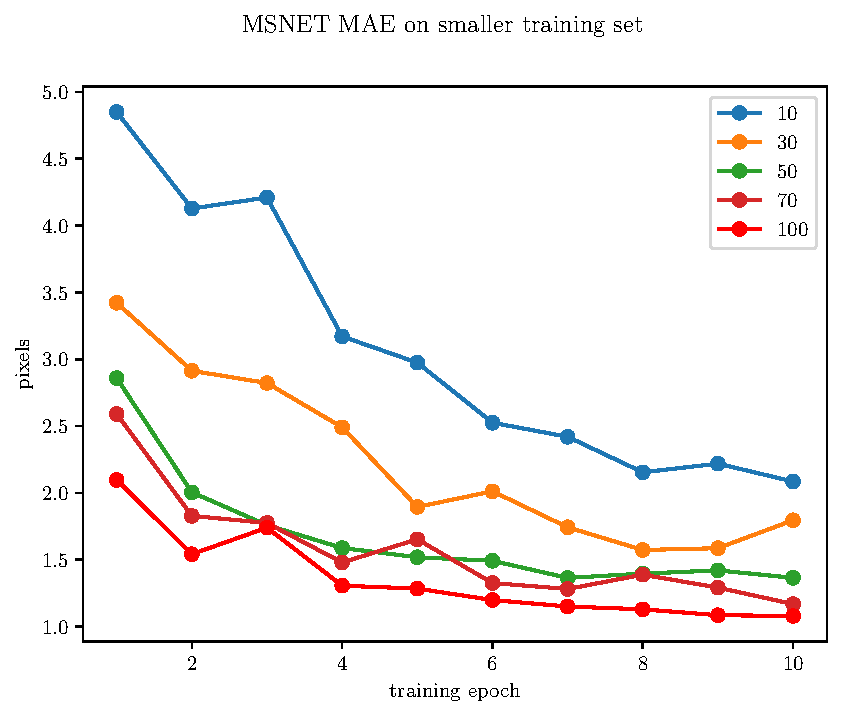
\includegraphics[width=0.49\textwidth]{figures/freiburg_msnet_mae_smaller_training_set.pdf}
    \caption{(Left) MSNet accuracy for different scale combinations. On the x-axis, there are the different scale combinations (i.e. the blue area contains single-scale set-ups, the green area two-scale, the purple area three-scale and the orange area the four-scale combination that was used in the training phase). On the first row we observe the $\mu$ and $\sigma$ of the absolute end-point error and on the second row the $\mu$ and $\sigma$ of the percentage of points with end-point error over 3 pixel.}
    \label{fig:msnet_scales_evaluation}

\end{figure}

\subsection{Multi-Scale fusion analysis} \label{sec:4_1}

In this section, we provide a qualitative illustration of how MSNet gradually adopts the information from coarse to fine scales.

In figure \ref{fig:multiscale_importance}, we focus on the \textit{MultiScaleFusion} algorithm. We choose two regions with different properties; the yellow-box region contains a thin object with rich texture, appropriate for a small, fine-scale patch. Conversely, the orange-box contains a background wall with a repetitive pattern, appropriate for a large, coarse-scale patch. We verify that the single-scale predictions agree with our intuition; only fine-scales ($t=2^2, t = 2^3$) succeed in the yellow-box area, whereas only coarse-scales succeed in the orange area ($t =2^4, t=2^5$). 

The multi-scale prediction succeeds in both scenarios. In the yellow-box area, the model initiates with an erroneous prediction from the coarse-scale $t=2^5$, but it gradually esteems the (most accurate) fine-scales. In the orange-box, where the initial prediction $t=2^5$ is accurate, the model remains unaffected by the erroneous coarse-scales. 

In figure \ref{fig:EMAPs}, all the single and multi-scale predictions of a single example (from the test set) are presented accompanied by their corresponding error images. We observe that the prediction procedure follows a step-by-step refinement of the initial low-resolution prediction; initially, the network predicts a rough coarse-scale estimation of the depth. As it explores the fine-scales, it gradually adopts high-resolution details for producing the final disparity map.

\begin{figure}[htb!]
    \begin{center}
        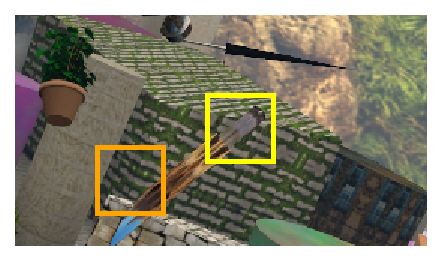
\includegraphics[width=0.5\textwidth]{paper/latex/figures/multiscale_importance_image_patches.pdf}\\
        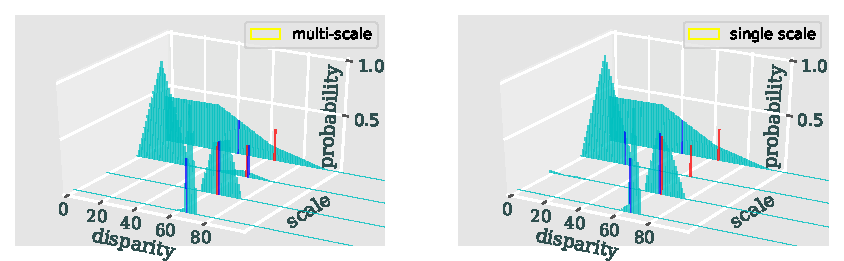
\includegraphics[width=0.9\textwidth]{paper/latex/figures/multiscale_importance_graph_high_resolution.pdf}\\
        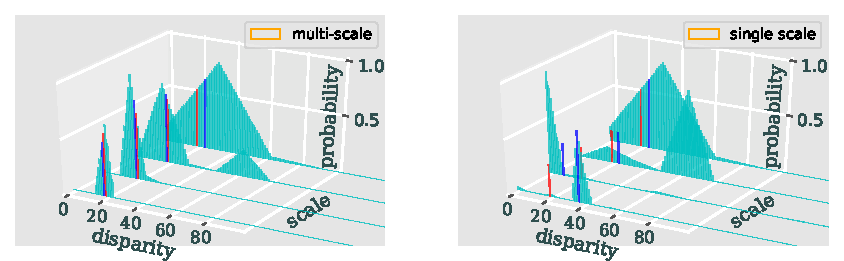
\includegraphics[width=0.9\textwidth]{figures/multiscale_importance_graph_low_resolution.pdf}
    \end{center}
    
    \caption{Comparison of two different areas of the image. The first row is related to the yellow box and the second one to the orange box. In all graphs, we observe the probabilities attached to each disparity under consideration. The blue line is the predicted disparity, after the $softargmax$ operator is applied, and the red line is the ground-truth disparuty. The single-scale graphs (right column) the prediction is done at each scale separately. Conversely, in the multi-scale graphs (left column) the prediction is based incrementally to more scales; $\hat{Y}^{t_0 = 2^5}$ ... to $\hat{Y}^\{t_0=2^2, ... t_3 = 2^5\}$ from back-to-forward}
    \label{fig:multiscale_importance}
\end{figure}


\section{Conclusion and Future Work}

In this paper, we proposed a scalable CNN model, that can be tuned for efficiency or accuracy according to the requirements of each application. For achieving this agility, we designed and trained all the learnable parts of the model in scale-independent tasks (feature extraction, combining information in pairs of two processing scales etc.), which enables specifying the processing scales at inference time. We confirmed that in general terms, our model has learned to exploit the accurate sub-regions from each processing scale and discard the erroneous ones. We also observed that reinforcing multi-scale processing explicitly leads to superior performance compared to the models that enable multi-scale implicitly. Finally, our method exhibits competitive results compared to the State-of-the-art methods in the SceneFlow dataset, even though it involves significantly less learnable parameters.

There are, of course, some open questions to be examined in the future. We proposed that the most significant advantage of our method is the ability to define the processing scales at test time.  Nevertheless, we provide no tool for answering two critical questions; (a) how many and (b) which specific scales to use according to the properties of the input. Hence, the scale specification depends upon how many computational resources we have available and whether we target mostly on accuracy or efficiency. However, since the correct set of processing scales depend on the qualitative characteristics of the stereo pair, it should be possible to determine them automatically; future work could focus on this exploration.

\clearpage
\bibliographystyle{splncs}
\bibliography{egbib}
\end{document}